Having presented an approach for constructing query processing architectures through assembly-based modularity,
in this chapter, we demonstrate its flexibility by applying it to a number of use cases and applications.
More specifically:

\begin{itemize}
  \item We demonstrate how both a document and a term-partitioned secondary
  index can be implemented using QPU-based architectures (section~\ref{sec:cs_index_partitioning}).
  In addition,
  we use this case study to describe in detail the construction and functionality of QPU graph,
  including the configuration of query processing units, and the queries sent between units
  during initialization and query processing.

  \item We examine a state-of-the-art approach to providing federated metadata search over data spread
  across multiple private and public cloud storage platforms,
  and propose a decentralized approach that places index entries closer to the corpus in order to improve
  freshness (section~\ref{sec:zenko}).
  Moreover, we present a QPU architecture that implements partial index replication.
  This approach provides fine-grained control over the placement of index entries:
  Heavily queries index entries are placed closer to the users,
  while heavily update are placed closer to the corpus

  \item We examine a read-heavy news aggregator application,
  and propose a QPU-based query processing system for maintaining pre-computed state in order to improve the application's performance,
  while simplifying its code (section~\ref{sec:lobsters}).
  To achieve that, we present a QPU that implements partial materialization in materialized views:
  Only materialized view entries expected to be requested by the application are materialized.
  This reduces the view's memory footprint as well as the volume communication required for keeping view entries up-to-date
  with the corpus.
  Furthermore, we demonstrate how a QPU-based architecture can be distributed between data center and edge nodes,
  and use partial materialization to ensure that only heavily queried materialized view entries are placed at the edge.
\end{itemize}

\section{Flexible secondary index partitioning}
\label{sec:cs_index_partitioning}

As described in section~\ref{sec:index_partitioning_background}, the two main index partitioning schemes are:
\begin{itemize}
  \item \textbf{Partitioning by document}.
  Each index partition is responsible for the data items of a certain corpus partition,
  and is co-located in the same node as that corpus partition.
  \item \textbf{Partitioning by term}.
  Each index partition is responsible for a partition of the \textit{value space} of the indexed attribute;
  The placement of index partitions is independent from the placement of corpus partitions.
\end{itemize}

Experimental comparison of the two approaches \cite{dsilva:tworings, kejriwal:slik} has shown that there is no ``one-size-fits-all'' approach to secondary index partitioning.
Rather, each approach caters to different needs.
More specifically, partitioning by document is more suitable for:
\begin{itemize}
  \item Workloads with low selectivity queries, that return large result sets.
  \item Skewed distributions, in which a large number of data items correspond to a few attribute values.
  \item Write-intensive workloads that require low write latency.
\end{itemize}
\noindent
On the other hand, partitioning by term is more suitable for:
\begin{itemize}
  \item Large-scale systems with a large number of corpus partitions.
  \item High selectivity query workloads.
  \item Less skewed value distributions.
\end{itemize}

Because of that, applications can benefit from partitioning schemes adjusted to their data and workload characteristics.

In most existing query processing systems,
the choice of index partitioning scheme is made during the system's design, and is not configurable
by applications.
For example, MongoDB \cite{coubase:mongoindexes}, Cassandra \cite{cassandra:secondaryindexing} and Riak \cite{riakv:secondaryindexes}
only use the partitioning by document approach,
while HBase \cite{hbase:secondaryindexes} uses the partitioning by term approach.

In this section, we demonstrate the flexibility of the QPU-based query processing architecture by showing how it can be used to
be used to express both index partitioning schemes.
More specifically,
we present a QPU architecture that implements a document-partitioned index,
and one that implements a term-partitioned index.

The design of the QPU architectures that we present is based on observations about the properties of the two index partitioning schemes.
We categorize these observations using the derived state read and write path framework presented in
section~\ref{sec:read_write_path}:
\begin{itemize}
  \item In the partitioning by document scheme,
  the index \textbf{write path} is \textit{local}:
  An index partition receives updates only from the corpus partition it is co-located with.
  On the other hand, in the partitioning by term scheme,
  the write path involves a many-to-one relationship:
  An index partition receives from all corpus partitions updates that belong in the value space it is responsible for.

  \item In the partitioning by document scheme,
  the \textbf{read path} is a \textit{broadcast} operation,
  while partitioning by term
  only index partitions with relevant index entries are involved in processing a given query.
\end{itemize}

We present QPU architectures for the two index partitioning approaches using the photo album example of section~\ref{sec:read_write_path} as a reference.
The corpus is composed of a set of image files.
Each image is identified by a primary key, and is associated with a set of user-defined tags.
The corpus is partitioned using a hash of the primary key as the partitioning key.
An application needs to create a secondary index on the $predominantColor$ tag, which can be assigned values in the range $[\#000000$, $\#FFFFFF$].

Figures~\ref{fig:index_partitioned_by_document} and~\ref{fig:index_partitioned_by_term} show the QPU graphs for a
document-partitioned index and a term-partitioned index respectively, and their placement across system nodes.
For simplicity we assume that the number of corpus partitions is equal to the number of system nodes,
and that a corpus partition is placed on each node.

The two architectures have a number of general characteristic in common.
In both architectures, a Corpus Driver QPU is placed on each node,
and is responsible for the corresponding corpus partition.
It provides the QPU graph with access to the data items in that corpus partition,
as well as the updates performed on those data items.
In addition, an Index QPU is used to represent each index partition;
A partition Manager QPU is connected to all index partitions,
and is responsible for coordinating query access to them.

In sections~\ref{sec:cs_index_partitioning_write_path} and~\ref{sec:cs_index_partitioning_read_path} we describe
how the two QPU architecture achieve the write and read path properties described above:

\subsection{Write path}
\label{sec:cs_index_partitioning_write_path}

\begin{figure}
  \begin{minipage}{.5\textwidth}
    \centering
    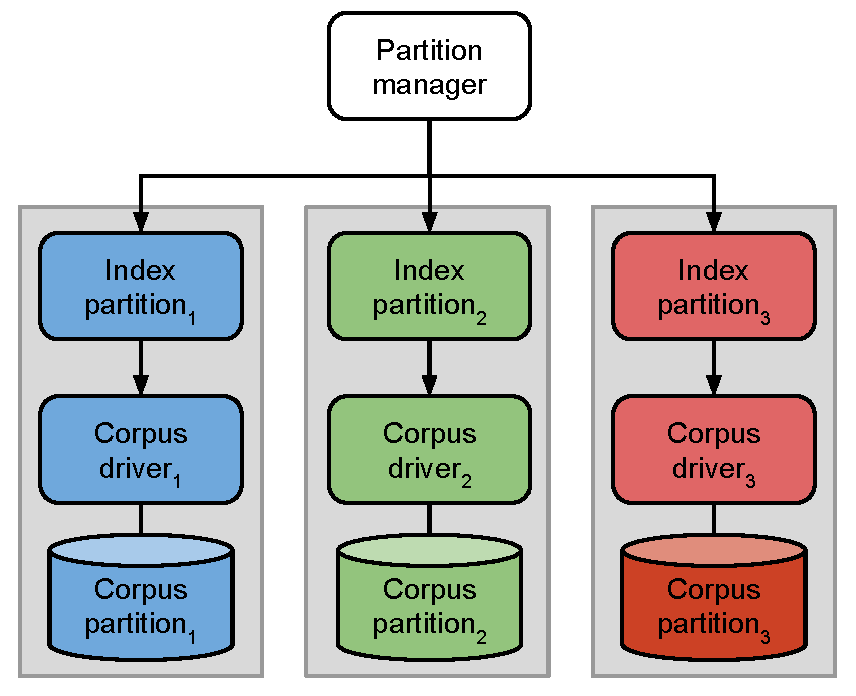
\includegraphics[scale=0.5]{./figures/case_studies/index_partitioned_by_document.pdf}
    \caption{QPU architecture for a document-partitioned secondary index.}
    \label{fig:index_partitioned_by_document}
  \end{minipage}%
  \begin{minipage}{.5\textwidth}
    \centering
    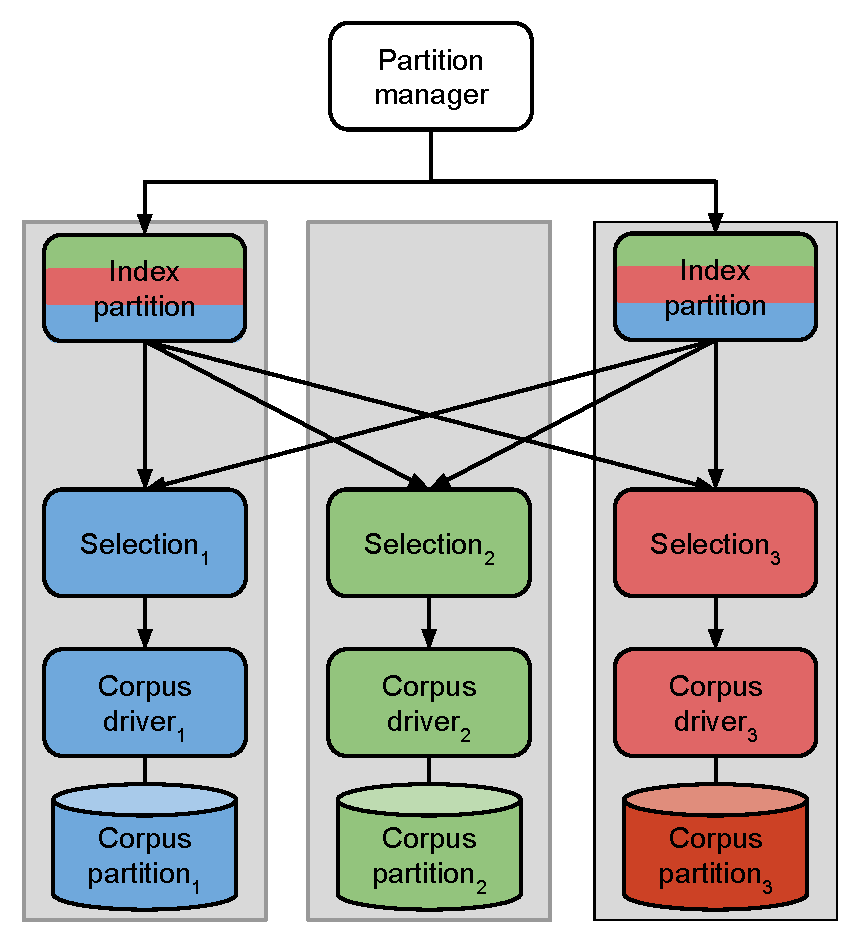
\includegraphics[scale=0.5]{./figures/case_studies/index_partitioned_by_term.pdf}
    \caption{QPU architecture for a term-partitioned secondary index.}
    \label{fig:index_partitioned_by_term}
  \end{minipage}
\end{figure}

The write path properties described above are achieved through (1) the QPU graph topology and the placement of graph vertices across system nodes,
and (2) the configuration of the Index QPUs (index partitions).

\subsubsection{Graph topology and placement}

\medskip
\noindent
\textbf{Partitioning by document.}
In the partitioning by document approach, we place an Index QPU on each system node,
and connect it to the corresponding Corpus Driver QPU.
As a result, each index partition has access corpus partition it is co-located with,
and therefore constructs and maintains an index containing the data items that belong in the corpus partition.

\medskip
\noindent
\textbf{Partitioning by term.}
In the partitioning by term approach,
we connect each Corpus Driver QPU to a Selection QPU,
and connect each Index QPU to all Selection units.
A Selection QPU forwards each update to the relevant index partition,
based on the attribute value in the update.
We describe in detail how this is achieved in the following section.
\subsubsection{Index partition configuration and graph initialization}

When the QPU graph for one of the partitioned index architectures is initialized,
the initialization method of each Index QPU sends a persistent query to the QPU's downstream connection,
in order to establish an input stream of updates (the initialization method of the Index QPU is presented in section~\ref{sec:qpu_class_examples}).
This downstream query is generated by the initialization method according to the QPU's configuration.
More specifically, each index QPU is configured with an attribute ($predominantColor$ in this example),
and an \textit{interval of values} of that attribute.
The index partition is responsible for index entries that correspond to attribute values in the specified interval.

In the partitioning by document approach,
each index partition is configured to be responsible for the entire attribute value space,
which in the photo album example is $[\#000000$, $\#FFFFFF$].
As a result, upon initialization, each index partition sends the query:

\begin{lstlisting}[caption={Query sent during initialization from each index partition to the corresponding Corpus Driver QPU,
  in the QPU graph shown in Figure~\ref{fig:index_partitioned_by_document}.}]
SELECT primaryKey, predominantColor
FROM photoAlbum
INTERVAL FROM LATEST
\end{lstlisting}

\noindent
to the Corpus Driver QPU it is connected to.
This initiates a stream between each Corpus Driver QPU and the corresponding Index QPU
The Corpus Driver initially sends a snapshot of the corresponding corpus partition to the
Index QPU, and then sends a stream record for each corpus update.

Conversely, in the partitioning by term approach, each index partition is responsible for a non-overlapping subset of the
attribute value space.
A simplified version of the configuration of the index partitions of the term-partitioned index QPU architecture
(figure~\ref{fig:index_partitioned_by_term}) is depicted below: \\

\begin{minipage}{.45\textwidth}
\begin{lstlisting}[
  language=json,
  caption={Configuration of the $index$ $partition_1$ in Figure~\ref{fig:index_partitioned_by_term}}
]
{
  // other configuration parameters
  "indexConfiguration": {
    "table": "photoAlbum",
    "attribute":
        "predominantColor",
    "lower_bound": #000000,
    "upper_bound": #7FFFFF
  }
}
\end{lstlisting}
\end{minipage}\hfill
\begin{minipage}{.45\textwidth}
\begin{lstlisting}[
  language=json,
  caption={Configuration of $index$ $partition_2$ in Figure~\ref{fig:index_partitioned_by_term}},captionpos=b
]
{
  // other configuration
  // parameters
  "indexConfiguration": {
    "table": "photoAlbum",
    "attribute":
        "predominantColor",
    "lower_bound": #7FFFFF,
    "upper_bound": #FFFFFF
  }
}
\end{lstlisting}
\end{minipage}

\medskip
\noindent
As a result, upon initialization, $index$ $partition_1$ sends the query:

\begin{lstlisting}[
  caption={Query sent during initialization from $index$ $partition_1$ to to each Selection QPU
  in the QPU graph shown in Figure~\ref{fig:index_partitioned_by_term}}
]
SELECT primaryKey, predominantColor
FROM photoAlbum
WHERE predominantColor >= #000000 AND predominantColor < #7FFFFF
INTERVAL FROM LATEST
\end{lstlisting}

\noindent
to each downstream Selection QPU, and $index$ $partition_2$ sends the query:

\begin{lstlisting}[
  caption={Query sent during initialization from $index$ $partition_2$ to to each Selection QPU
  in the QPU graph shown in Figure~\ref{fig:index_partitioned_by_term}}
]
SELECT primaryKey, predominantColor
FROM photoAlbum
WHERE predominantColor >= #7FFFFF AND predominantColor <= #FFFFFF
INTERVAL FROM LATEST
\end{lstlisting}

\noindent
to each downstream Selection QPU.

\noindent
As a result of receiving one the above queries,
each Selection QPU sends to each downstream Corpus Driver QPU the query:

\begin{lstlisting}[
  caption={Query sent during initialization from each Selection QPU each Corpus Driver QPU
  in the QPU graph shown in Figure~\ref{fig:index_partitioned_by_term}}
]
SELECT primaryKey, predominantColor
FROM photoAlbum
INTERVAL FROM LATEST
\end{lstlisting}

\noindent
As a result, each Selection QPU receives an input stream from the corresponding Corpus Driver QPU,
for each of the two above queries,
and filters the received streams according to the predicate specified by each query.
Therefore, $index$ $partition_1$ receives from all three corpus partitions first a snapshot and then updates
corresponding to the $predominantColor$ in the interval $[\#000000$, $\#7FFFFF)$.
Similarly, $index$ $partition_2$ receives stream records corresponding to the $predominantColor$ in the interval
$[\#7FFFFF$, $\#FFFFFF)$.

For example, given a update that inserts to the corpus an image file with $predominantColor$ $=$ $\#613930$, assigned to to $corpus$
$partition_2$, $Corpus$ $Driver_2$ sends to $Selection_2$ a record encoding that update.
This input record matches the query:

\begin{lstlisting}[
  caption={Query that retrieves image files from the $photoAlbum$ table based the value of the $predominantColor$ attribute}
]
SELECT primaryKey, predominantColor
FROM photoAlbum
WHERE predominantColor >= #000000 AND predominantColor < #7FFFFF
INTERVAL FROM LATEST
\end{lstlisting}

\noindent
and thus the $Selection_2$  forwards the record only to $index$ $partition_1$.

\subsection{Read path}
\label{sec:cs_index_partitioning_read_path}

In both QPU architectures, the Partition Manager QPU is connected to all Index QPUs.
As described in section~\ref{sec:qpc_tree}, given a query,
the Partition Manager's query processing method determines which downstream connections need to be contacted.
It generates the corresponding downstream queries using the domain trees of its downstream connections.

More specifically, given a query,
the query processing method, generates a query parse tree,
and performs an intersection between the query parse tree and the domain tree of each of its downstream connections.
The result of each intersection operation is a query parse tree of the downstream query to be sent to the corresponding
connection.
If the intersection result is empty, then the QPU does not send a downstream query to that connection.

\begin{figure}
  \centering
    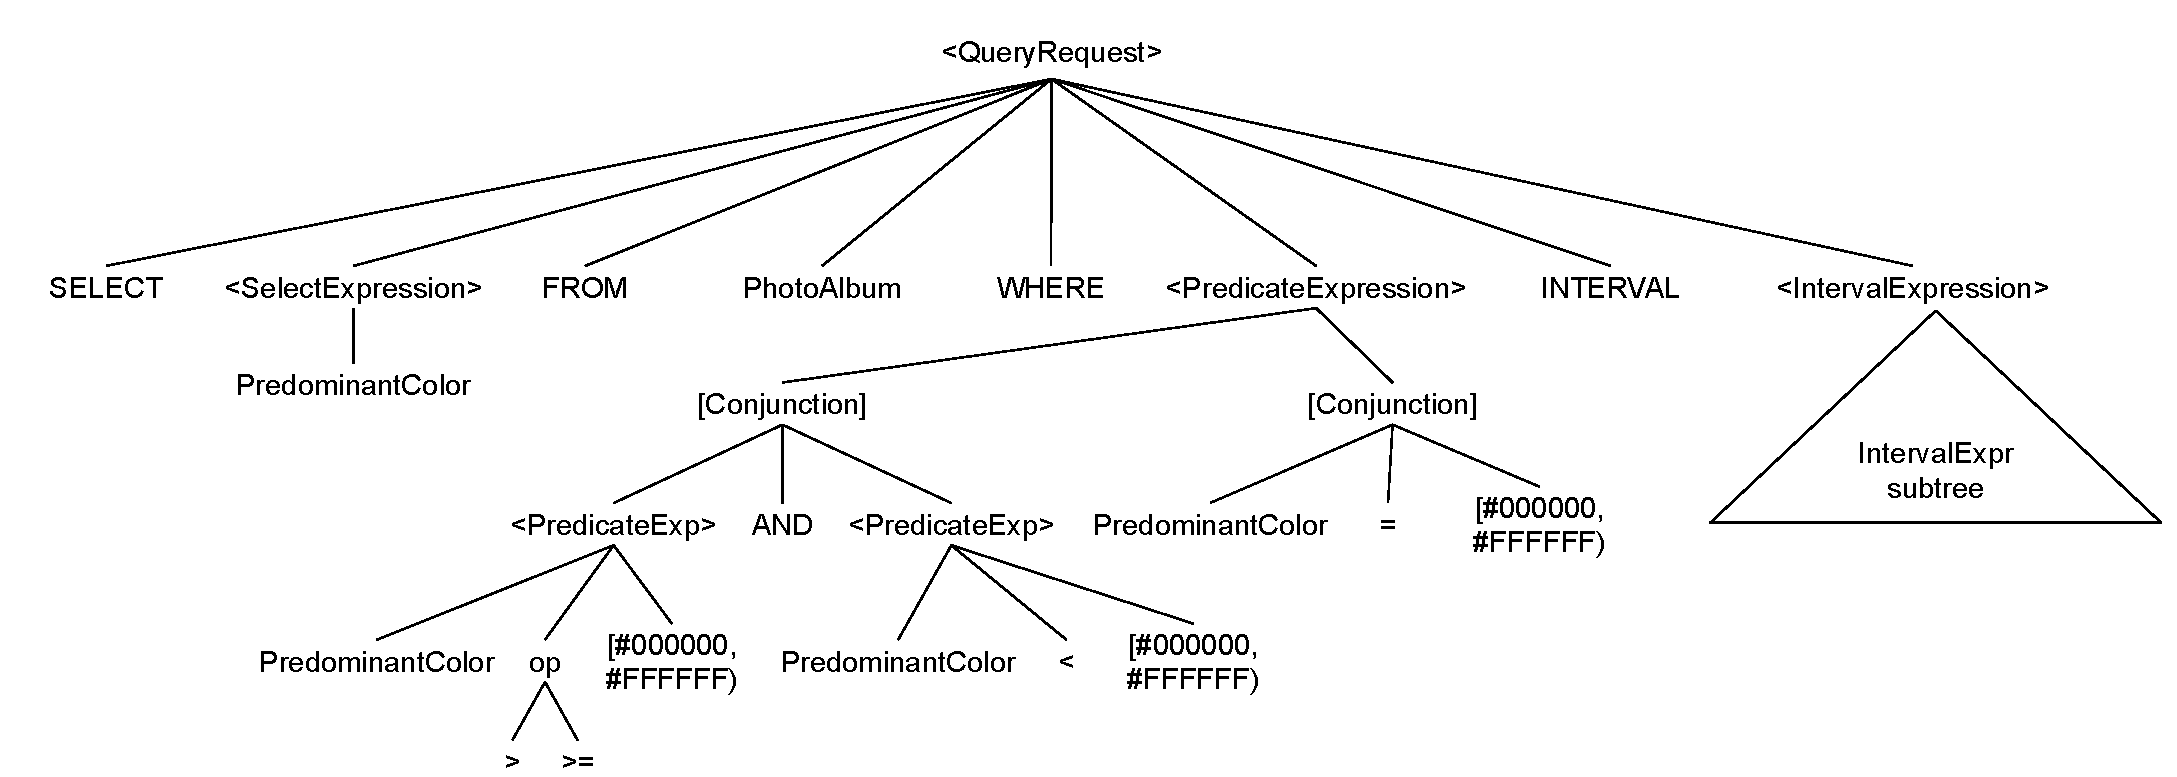
\includegraphics[width=\textwidth]{./figures/case_studies/qpt_index_partitioning_docs.pdf}
  \caption{Domain tree of an index partition in the document-partitioned index QPU architecture.}
  \label{fig:qpt_index_partitioning_docs}
\end{figure}

\medskip
\noindent
\textbf{Partitioning by document.}
The domain tree for an index partition in the document-partitioned index QPU architecture is shown in Figure~\ref{fig:qpt_index_partitioning_docs}.
As describe above, in the document-partitioned index, each index partition is responsible for the entire attribute value space of
the data items of one corpus partition.
The domain tree of every index partition is thus are the same as the one depicted in Figure~\ref{fig:qpt_index_partitioning_docs}.
Moreover, because this tree corresponds to the entire attribute value domain,
the intersection with any query parse tree is an identity function:
Performing an intersection between that domain tree a query parse tree leaves the parse tree unchanged.

Therefore,
given a query,
the Partition Manager QPU forwards the same query to each of its downstream connections.
This implements the required read path behavior.


\begin{figure}
  \begin{subfigure}{0.5\textwidth}
     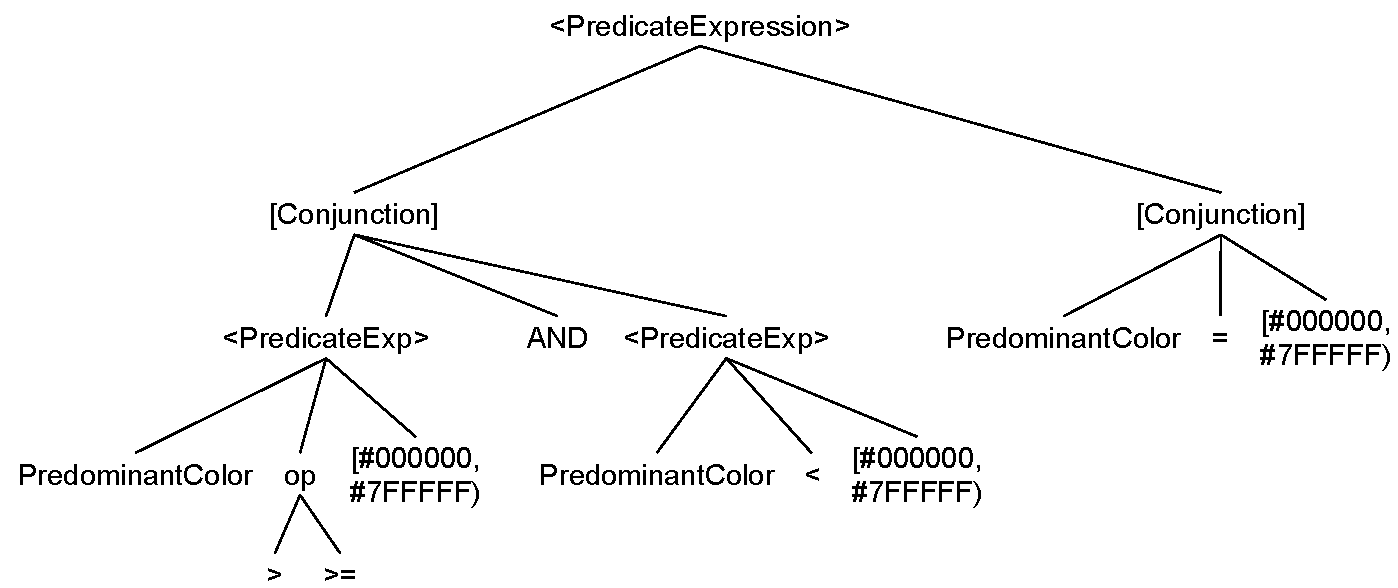
\includegraphics[width=\linewidth]{./figures/case_studies/qpt_index_partitioning_terms_1.pdf}%
     \caption{}
     \label{fig:qpt_index_partitioning_terms_1}
  \end{subfigure}%
  \hspace*{\fill}
  \begin{subfigure}{0.5\textwidth}
    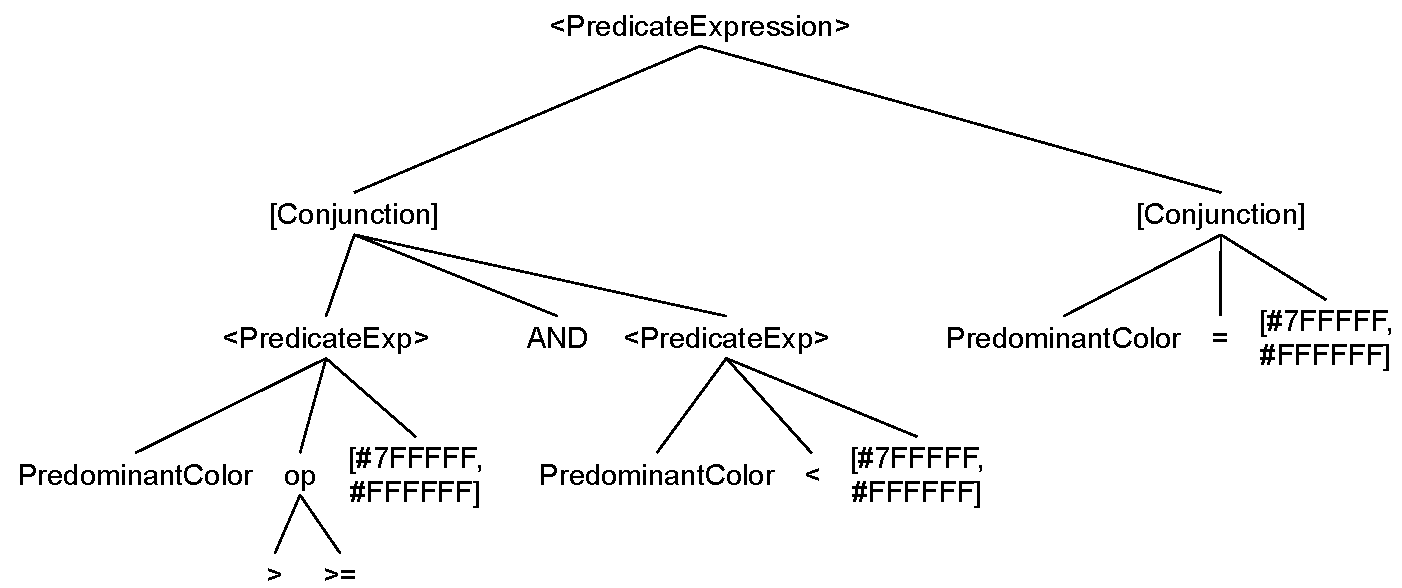
\includegraphics[width=\linewidth]{./figures/case_studies/qpt_index_partitioning_terms_2.pdf}%
    \caption{}
    \label{fig:qpt_index_partitioning_terms_2}
  \end{subfigure}%
\caption{The domain tree for $index$ $partition_1$ (\ref{fig:qpt_index_partitioning_terms_1}) and $index$ $partition_2$ (\ref{fig:qpt_index_partitioning_terms_2}) of the term-partitioned
index in Figure~\ref{fig:index_partitioned_by_term}}
\label{fig:qpt_index_partitioning_terms}
\end{figure}

% \begin{figure}
% \subfloat[]{%
% \centering
%   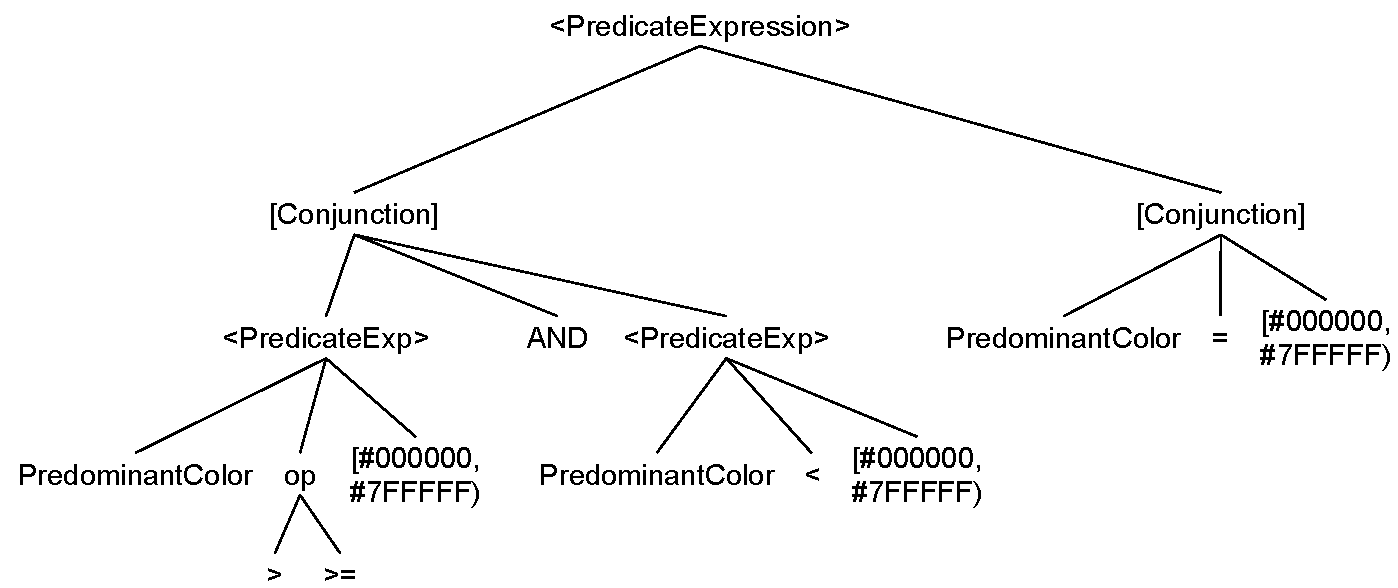
\includegraphics[width=0.6\textwidth]{./figures/case_studies/qpt_index_partitioning_terms_1.pdf}%
% }

% \subfloat[]{%
%   \centering
%   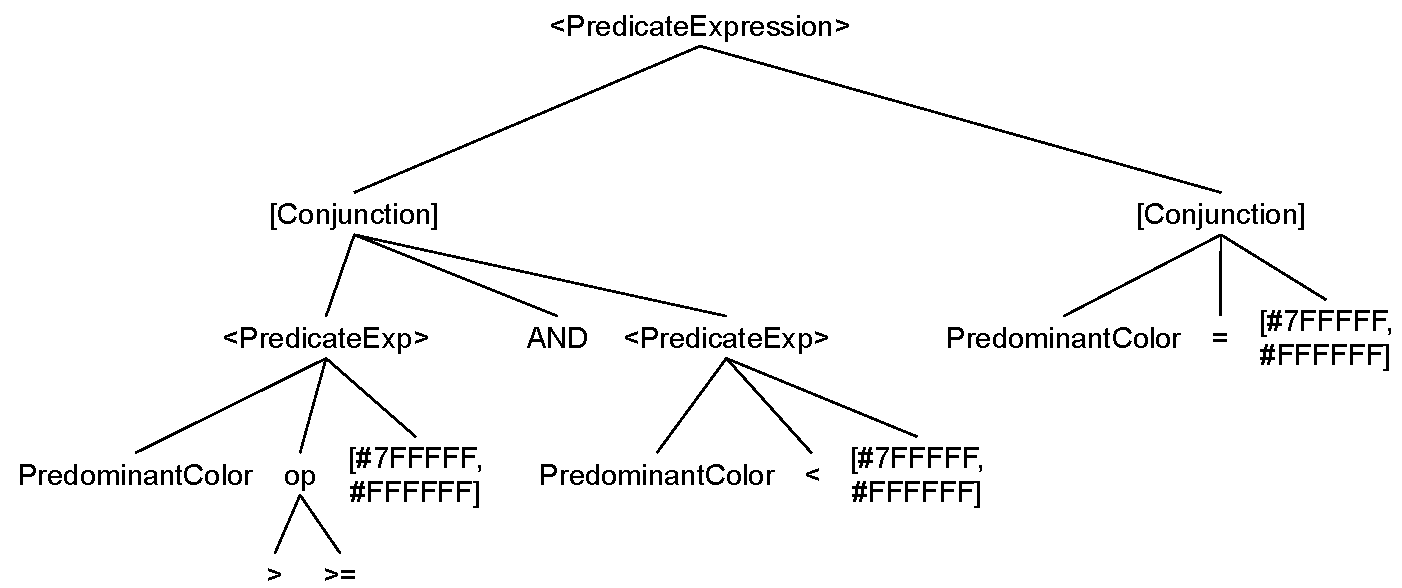
\includegraphics[width=0.6\textwidth]{./figures/case_studies/qpt_index_partitioning_terms_2.pdf}%
% }
% \caption{Domain tree for $index$ $partition_1$ (a) and $index$ $partition_2$ (b) of the term-partitioned
% index in Figure~\ref{fig:index_partitioned_by_term}}
% \label{fig:qpt_index_partitioning_terms}
% \end{figure}

\medskip
\noindent
\textbf{Partitioning by term}
Figure~\ref{fig:qpt_index_partitioning_terms} shows the $<predicateExpression>$ subtrees of the domain trees
for $index$ $partition_1$ and $index$ $partition_2$ in the term-partitioned index architecture.
The domain tree of $index$ $partition_1$ represents the set of queries in the interval $[\#000000$, $\#7FFFFF)$,
while the domain tree of $index$ $partition_2$ represents the interval $[\#7FFFFF$, $\#FFFFFF]$.

We describe how the term-partitioned index architecture processes queries by running through an example query.
Given the query:

\begin{lstlisting}[
  caption={Query that retrieves image files from the $photoAlbum$ table based the value of the $predominantColor$ attribute},
  label={lst:predominantcolor_q},
  ]
Q = SELECT primaryKey, predominantColor
    FROM photoAlbum
    WHERE predominantColor >= #21B1FF
    AND predominantColor < #ff7b75
    INTERVAL FROM LATEST
\end{lstlisting}

\noindent
the Partition Manager QPU calculates the intersection between the parse tree of $Q$ the domain tree of $index$ $partition_1$.
This results to the downstream query:

\begin{lstlisting}[
  caption={Sub-query sent from the Partition Manager QPU to $index$ $partition_1$ in Figure~\ref{fig:qpt_index_partitioning_terms}
  in order to process the query in Listing~\ref{lst:predominantcolor_q}.}]
Q1 = SELECT primaryKey, predominantColor
     FROM photoAlbum
     WHERE predominantColor >= #21B1FF
     AND predominantColor < #7FFFFF
     INTERVAL FROM LATEST
\end{lstlisting}

\noindent
Similarly, the downstream query for $index$ $partition_2$ is:

\begin{lstlisting}[
caption={Sub-query sent from the Partition Manager QPU to $index$ $partition_2$ in Figure~\ref{fig:qpt_index_partitioning_terms}
  in order to process the query in Listing~\ref{lst:predominantcolor_q}.}]
]
Q2 = SELECT primaryKey, predominantColor
     FROM photoAlbum
     WHERE predominantColor >= #800000
     AND predominantColor < #ff7b75
     INTERVAL FROM LATEST
\end{lstlisting}

\noindent
The Partition Manager QPU sends $Q1$ to $index$ $partition_1$ and $Q2$ to $index$ $partition_2$.
It then merges resulting input streams, and emits the merged stream as its output stream.

In summary, in the term-partitioned architecture,
the Partition Manager generates and sends downstream queries to index partitions according their corresponding
value intervals, using the domain tree mechanism.

In conclusion, we have described how the QPU-based composable query processing architecture can be used to construct both
document and term partitioned indexes.
Using this flexibility, a database system can support both partitioning schemes and provide applications the ability to
select the partitioning scheme of each indexes according the data distribution characteristics and the expected workload.

\begin{figure}
  \centering
    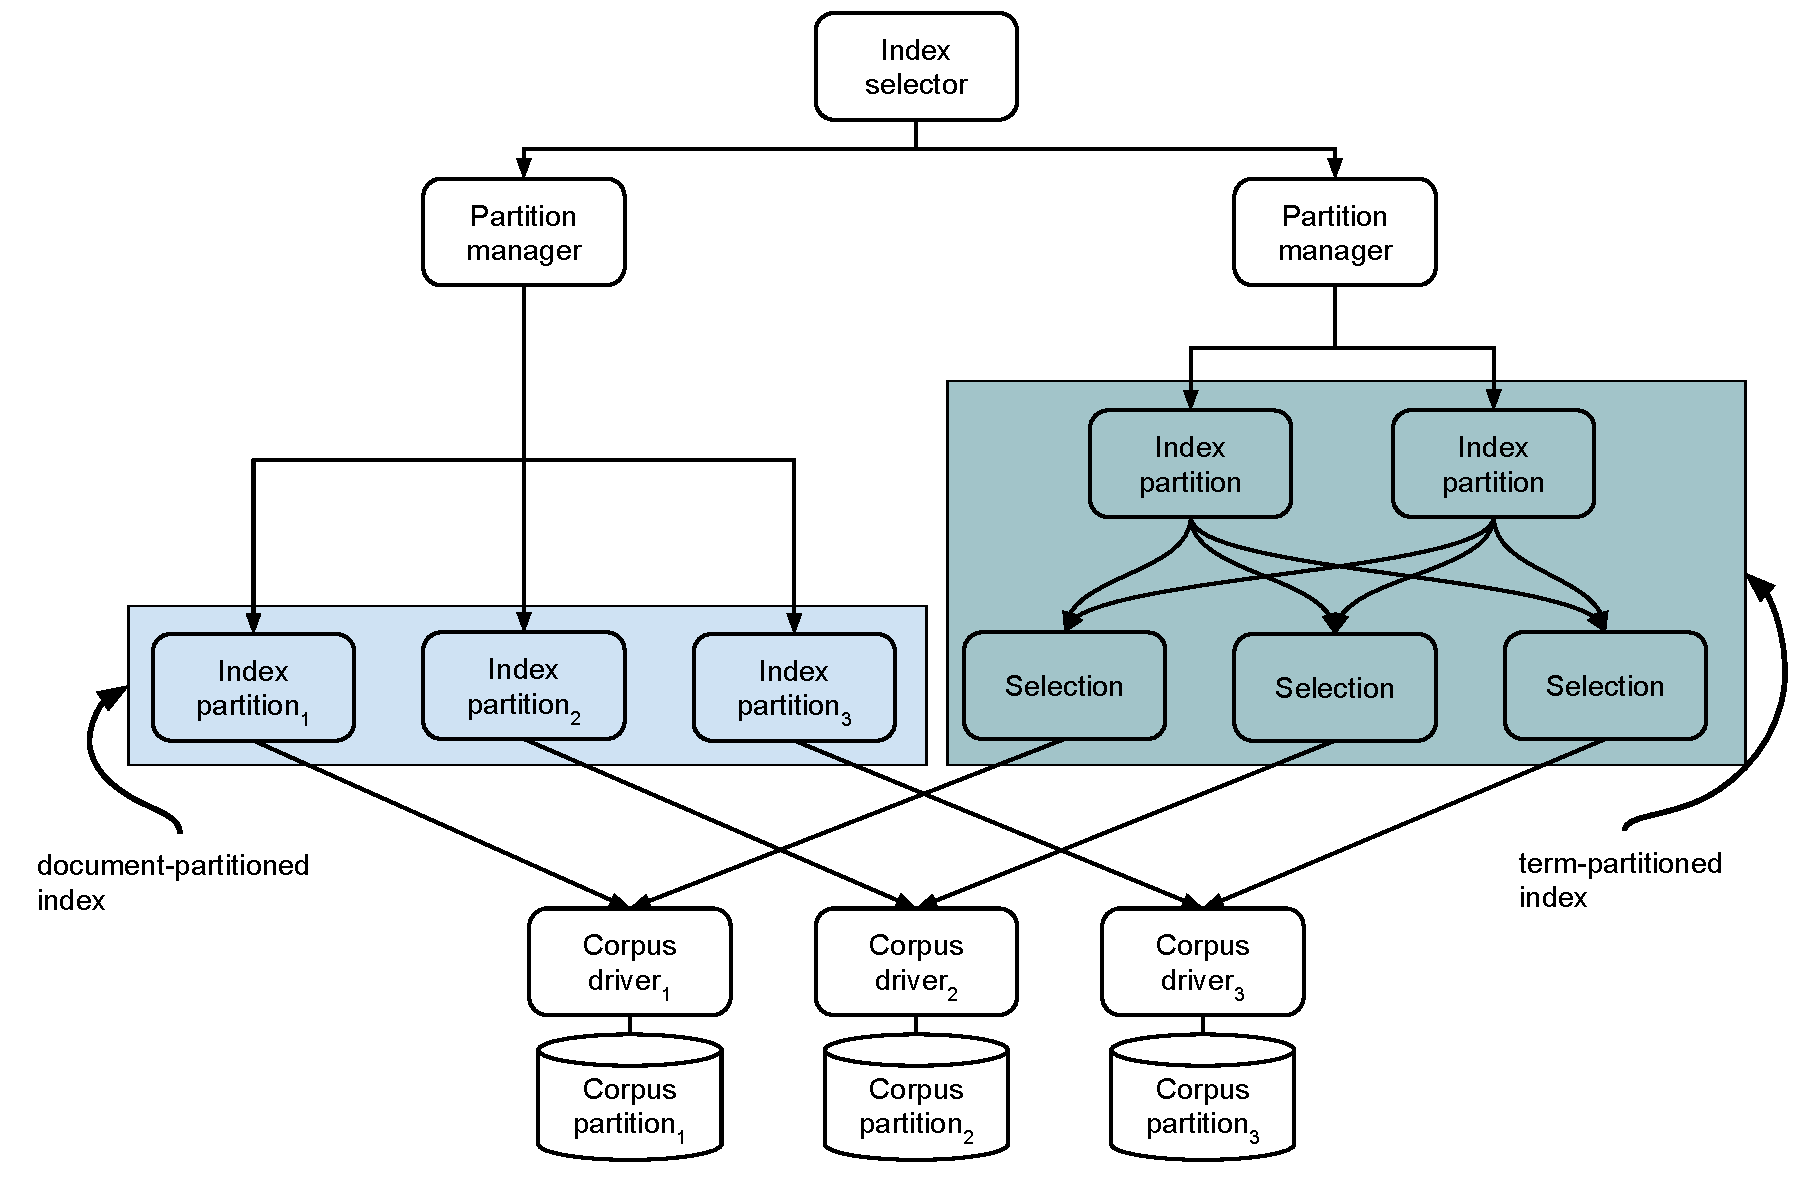
\includegraphics[width=\textwidth]{./figures/case_studies/index_partitioned_two_level.pdf}
  \caption{QPU architecture for a two-tiered partitioned index, composed of a document-partitioned, and a term-partitioned tier.}
  \label{fig:index_partitioned_two_level}
\end{figure}

It is important to note that some existing databases,
such as Amazon DynamoDB \cite{dynamodb:secondaryindexes} and Apache Phoenix \cite{phoenix:secondaryidnexing}
support both index partitioning schemes.
However, we believe that the proposed approach provides a more structured approach to the design of query processing systems,
and enables additional flexibility.

For example, using the QPU-based architecture we can construct a hybrid, two-tiered partitioned secondary index,
consisting of a document-partitioned tier and a term-partitioned tier, as shown in Figure~\ref{fig:index_partitioned_two_level}.
We configure the document-partitioned tier to be strongly consistent with the corpus,
by configuring each connection between an Index QPU and the corresponding Corpus Driver to be synchronous.
We configure the term-partitioned tier to be eventually consistent with the corpus,
by configuring each Index --- Corpus Driver connection as asynchronous.

The document-partitioned trades consistent query results with more limited query load scalability,
as each query needs to be forwarded to every index partition.
The term-partitioned index trades higher query load scalability, with potentially stale query results.

Using this query processing architecture, individual queries are able to choose between the two tiers
according to their requirements.
To achieve this, we introduce the Index Selector QPU class.
The Index Selector is responsible for managing access to the two index tiers,
by forwarding each query to one of the Partition Manager QPUs it connected to.
It selects between its connections based on an indication by the given query:
Queries can select between the two partitioned index tiers using a special ``control'' attribute, called $tier$.
The query:

\begin{lstlisting}[
  caption={Query that retrieves an image file from the $photoAlbum$ table based the value of its $predominantColor$ attribute.}
]
SELECT primaryKey, predominantColor
FROM photoAlbum
WHERE predominantColor = #ff7b75
AND tier = sync
\end{lstlisting}

\noindent
will be forwarded to the document-partitioned index, while the query:

\begin{lstlisting}[
  caption={Query that retrieves an image file from the $photoAlbum$ table based the value of its $predominantColor$ attribute.}
]
SELECT primaryKey, predominantColor
FROM photoAlbum
WHERE predominantColor = #ff7b75
AND tier = async
\end{lstlisting}

\noindent
will be forwarded to the term-partitioned index.

This architecture trades this functionality with the resources required for maintaining
two index replicas.

%%%%%%%%%%%%%%%%%%%%%%%%%%%%%%%%%%%%%%%%%%%%%%%%%%%%%%%%%%%%%%%%%%%%%%%%%%%%%%%%%%%%%%%%%%%%%%%%%%%%%%%%%%%%%%%%%%%%%%%%


\section{Federated secondary attribute search for multi-cloud object storage}
\label{sec:zenko}

While most enterprise data today originate from and is stored on-premises storage systems,
use cases for hybrid and multi-cloud storage are emerging in many industries.
For example, in the media industry, while the creation of content in on-premises private clouds is prevalent,
the use of public cloud services for content distribution and transcoding \cite{scality:bloomberg} is growing.
Moreover, organization increasingly choose to spread their data across multiple public cloud providers in order to avoid
dependence on a single provider, and improve their resilience against failures.

The advent of data distributed across multiple independent storage platforms has created the need for unified access to data across platforms.
In this section, we examine Zenko \cite{zenko:docs}, a multi-cloud data controller that aims to address this need.
Zenko provides a common namespace over a set of distinct object storage platforms,
including Amazon S3, Microsoft Azure Blob storage, and Google Cloud Storage.
It allows applications to access data in multiple storage locations using the AWS S3 API \cite{aws:s3}.

We focus on Zenko's federated metadata search functionality \cite{zenko:mdsearch}.
It is common for application to mark objects with metadata tags.
Zenko provides applications the ability to retrieve objects based on queries on their metadata tags,
independent from storage location.

Zenko uses a warehousing approach to provide federated metadata search:
It integrates metadata tags for objects stored on all storage platforms in a central \textit{metadata store} \cite{zenko:architecture, zenko:mongodb}.
More specifically, it uses a MongoDB deployment as this metadata store.
MongoDB provides the ability to create indexes on document attributes,
and to retrieve documents using queries on these attributes.
Zenko uses this functionality to implement metadata search:
Object metadata are stored as documents in MongoDB.
Queries on metadata tags are translated to MongoDB find requests.

A typical Zenko deployment consists of Zenko along with a private storage system deployed on-premises,
and multiple public cloud storage platforms, each on a different data center.
For this case study, we refer to each data center / storage system as a \textit{storage location}.
The primary data access method is through Zenko's API:
Application communicate with Zenko to read and write objects,
and Zenko is responsible for storing and retrieving each object from the corresponding storage location according to a specified policy.
In addition,
applications can write directly to some of the storage systems.
Zenko ingests updates performed directly to an underlying storage system through a mechanism called out-of-band updates \cite{zenko:outofband}.

In this case study,
we present an alternative approach for supporting federated metadata search on object storage platforms.
More specifically, we demonstrate how the QPU-based query processing architecture can be used to construct
a \textit{decentralized} secondary index that federates data stored on multiple storage locations;
The main idea is to partition the secondary index based on the storage location of each object,
and place each index partition close to the corresponding data.

There are two main advantages to this approach compared to the warehousing approach:
\begin{itemize}
  \item It ensures that the write path of the index does not require cross data center communication.
  This means that the system can update index partitions synchronously without the prohibitive overhead of
  cross data center communication.
  Alternatively, if index maintenance is asynchronous,
  the index can by updated in a more timely fashion, resulting in less stale index entries.
  In general, a decentralized index is better suited for applications that require up-to-date query results.

  \item By being distributed across multiple data centers,
  the query processing system can remain available in the face of a data center failure.
\end{itemize}

We make two assumptions:
The first is that storage platforms used in this case study have a common, object storage data model.
Second, a Corpus Driver QPU is available for each storage platform.
This assumptions ensure that a QPU graph can be connected with multiple underlying storage systems.

The QPU architecture for the multi-cloud index is shown in Figure~\ref{fig:federated_index} (a).
We built on the partitioned index QPU architectures presented in Section~\ref{sec:cs_index_partitioning}.
We construct a partitioned index QPU graph for each storage system, and co-locate it in the same data center as that
storage system.
We refer to each of these QPU graphs as an \textit{index location}.
Each index location is independent and can be constructed using either the partitioning by document or partitioning by
term approach.
In addition, a Partition Manager QPU is deployed on each storage location,
and connected to all index locations.
The Partition Manager QPUs consist the root nodes of the QPU graph.
Given a query, a Partition Manager QPU forwards the same query to every index location,
and then merges the resulting input streams.
This approach is equivalent to the document-partitioned index approach.

\begin{figure}
  \begin{minipage}{.5\textwidth}
    \centering
    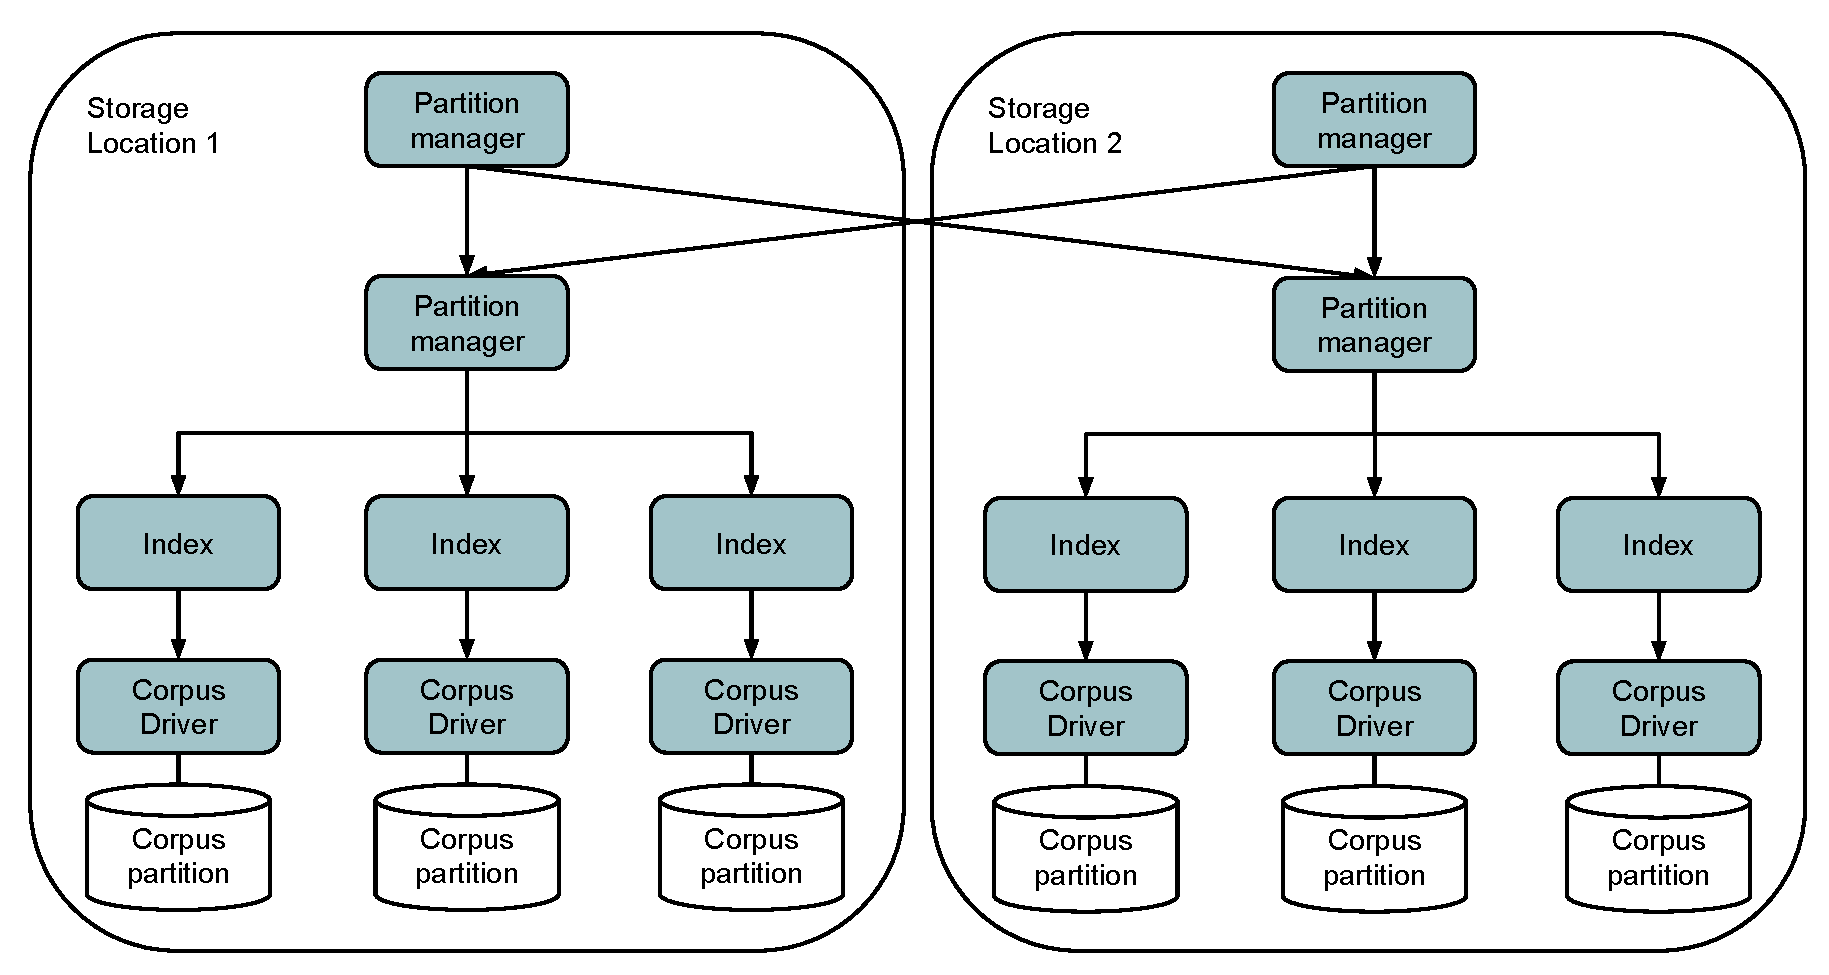
\includegraphics[scale=0.24]{./figures/case_studies/federated_index.pdf}
  \end{minipage}%
  \begin{minipage}{.5\textwidth}
    \centering
    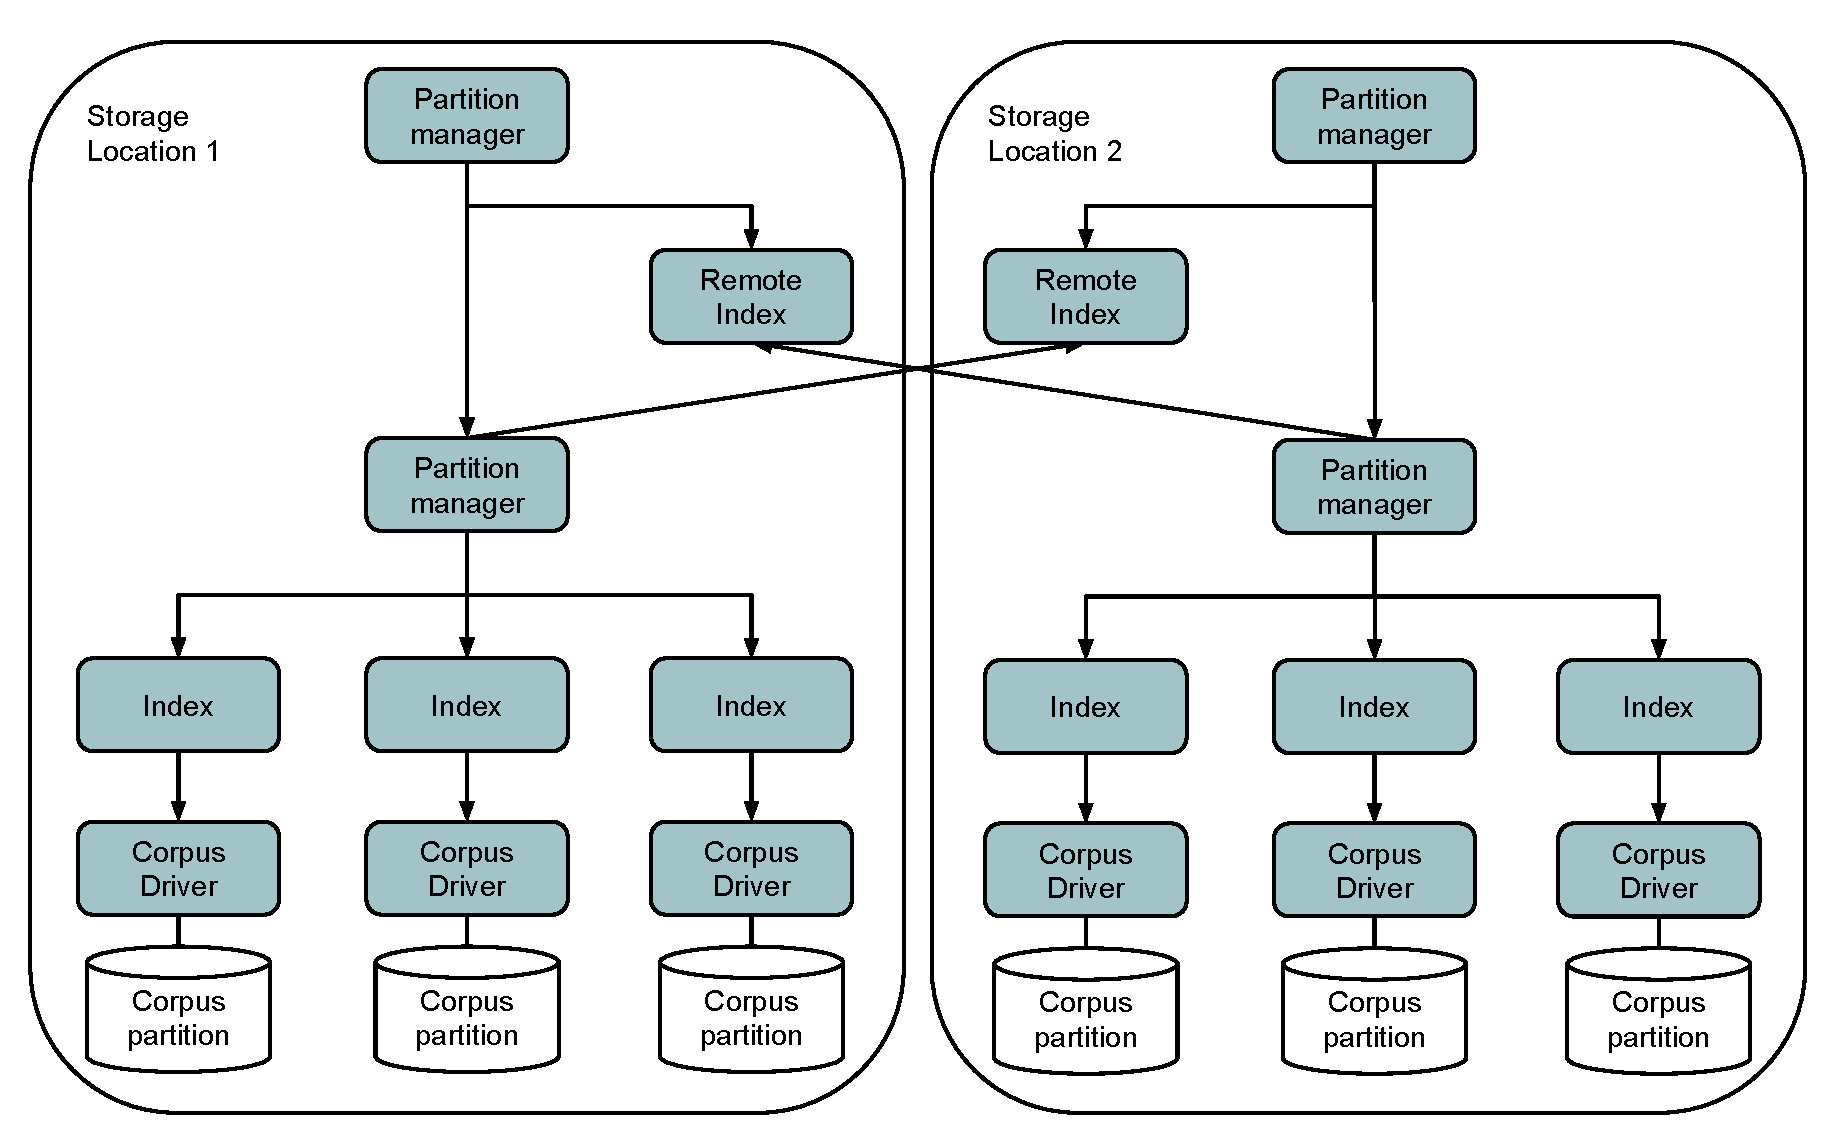
\includegraphics[scale=0.24]{./figures/case_studies/federated_index_remote.pdf}
  \end{minipage}
  \caption{QPU architecture for a secondary index that federates two storage locations.
  (a) Using a Partition Manager as a root at each storage location that forwards queries to every storage location.
  (b) Using \textit{partial index replicas} implemented by Partial Index QPUs.}
  \label{fig:federated_index}
\end{figure}

The downside of this approach is that the index query processing system needs to forward each query to every
storage location.

This can be addressed by replicating the entire index at each storage location,
but that would multiply the storage and memory footprint of the index.
In addition it would shift the requirement for cross data center communication to the write path;
Every update would need to be sent to every other data center.

We propose an alternative approach, based on partial index replication.
To achieve that, we introduce the Partial Index QPU class.
The goal of the Partial Index class is to implement secondary index in which only a subset of index entries are materialized,
essentially implementing a \textit{partial replica of a secondary index}.
The insight is that some index entries are accessed more frequently than others;
The Partial Index, similarly to a cache, materializes the most recently read index entries;
Additionally, it does not invalidate entries, but, similarly to an index, performs incremental updates to keep them up-to-date
with the corpus.
This has two benefits:
It bounds the memory footprint of the index, and reduces the cross data center communication needed by the index both in the read and the write path.
In the read path, queries that can be processed using materialized index entries do not need to be forwarded to
another storage location.
In the write path
Using the Remote Index QPU reduces the cross data center communication required for index processing by
replicating recently accessed index entries.

We use the Partial Index QPU to propose an improvement to the QPU architecture of Figure~\ref{fig:federated_index} (a).
We deploy Partial Index QPU on each storage location, and connected to the index sub-graph of the Partial index.
Each Partial Index QPU works as follows.
When initially deployed, it none of its entries materialized.
When it receives a query, its query processing method forwards the query to its downstream connection,
which in this QPU graph is an index location, as a persistent query.
It stores the received entries, incrementally updates them using the input stream of updates.
A difference with the Index QPU is therefore that the Partial Index establishes an input stream for each materialized
index entry, while the Index requires a single input stream.

While the partial index replication can potentially reduce the write path cross data center communication of an index replica,
it might still incur significant between storage locations,
in cases in which materialized index entries are updated frequently.
To address this issue,
we extend the Partial Index class with a mechanism for measuring the rate of updates to each index entry.
If the update rate for a certain entry crosses a threshold specified by the QPUs configuration,
then the QPU stops receiving updates for this entry and discards it.

The Partial Index QPU provides fine-grained placement of index entries.
Index entries that are queried more heavily are replicated, and thus placed closer to clients,
while index entries that are updated more heavily are placed closer to the corpus.

This technique has two benefits.
First it reduces the memory and storage resources required for query processing by partially replicating index entries.
Second, it reduces network resource consumption for data transfer between storage locations,
as each index entry is placed at the storage location it communicates more with.

The QPU architectures described in this case demonstrate an important property of QPU-based query processing architectures:
A QPU graph can have a hierarchical structure,
in which lower layers are composed composed of multiple independent sub-graphs,
which are then connected by higher layers.
Th federated index architecture consists the partitioned index for each storage location (lower layer),
connected by Partition Manager QPUs (higher layer).
Moreover, the lower layer is transparent to the higher layer.
For example, the lower layer of the federated index architecture can used either the partitioning by term or
partitioning by document approach without affecting the system's functionality.

\subsection{Predicate-based indexing}

In this section, we extend the multi-cloud index case study by examining a use case inspired by one of Scality's customers.
We consider the example of a media organization that operates broadcasting and streaming services.
It stores media assets (video content, images) used by these services in an object storage system.
As described above, objects are tagged with metadata tags;
Applications use queries on metadata tags to provide recommendation and user search functionalities.
The organization operates in two geographic locations, and a separate storage platform is used for each location.

The metadata search requirement of this use case are as follows:
Applications on each geographic location need low latency metadata search on \textit{local} corpus (data stored on that geographic location),
as well as a \textit{subset} of corpus in the remote location.
This subset is specified by the application, and is expressed as predicates on metadata tags.
In other words, for an application that operates in $location_A$, there is an ``interest set'' in $location_B$:
a subset of the corpus $location_B$ that the application accesses frequently and needs low latency metadata search on.

\begin{figure}
  \centering
    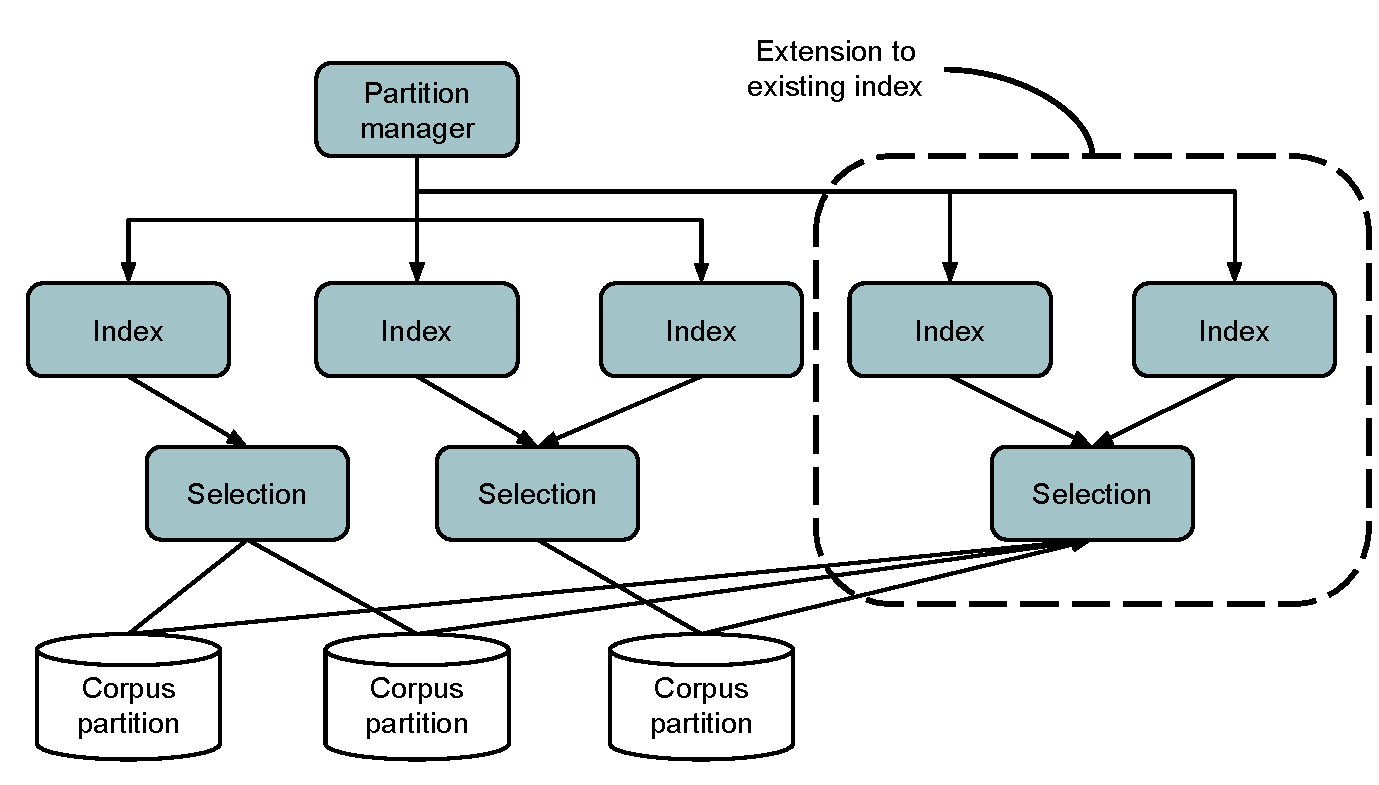
\includegraphics[width=0.7\textwidth]{./figures/case_studies/predicate_based_index.pdf}
  \caption{QPU architecture for a predicate-based secondary index.}
  \label{fig:predicate_based_index}
\end{figure}

While the state-of-the-art warehousing approach of constructing a central index with metadata tags from all objects
on both locations can be applied to achieve these requirements,
that would potentially use significantly more resources that required,
if the interest set is small compared to the corpus.

Instead, we construct a secondary index that indexes only the interest set,
by filtering the corpus based on a given predicate before indexing.
Figure~\ref{fig:predicate_based_index} shows the QPU architecture used to achieve that.
We use a layer of Selection QPUs between the corpus (Corpus Driver QPUs) and the partitioned index.
The Selection QPUs apply a filter on the corpus based on the query that defines the interest set,
making only data items that satisfy it available to the index.
We refer to this architecture, as an \textit{predicate-based secondary index}.

A property of this architecture is that it is extensible:
Additional corpus subsets can be added to the filtered index by deploying additional Selection --- Index QPU subgraphs,
and connecting them through a Partition Manager QPU.

A federated index QPU architecture for this use case consists of two parts
follows the same logic as the one presented in Figures~\ref{fig:federated_index} (a) and (b),
with the addition that in one of the two storage locations we use a predicate-based index.


%%%%%%%%%%%%%%%%%%%%%%%%%%%%%%%%%%%%%%%%%%%%%%%%%%%%%%%%%%%%%%%%%%%%%%%%%%%%%%%%%%%%%%%%%%%%%%%%%%%%%%%%%%%%%%%%%%%%%%%%
% \section{Materialized views at the edge}
\section{Materialized view middleware}
\label{sec:lobsters}

In this case study, we examine an existing application that requires the use of pre-computed state,
and study how it can benefit by using a QPU-based architecture for query processing.

Lobsters \cite{lobste:rs} is a news aggregator web application.
In Lobsters, users post and comment on links (\textit{stories} in the Lobsters terminology).
In addition, users vote on stories and comments, and votes are used to rank stories.

Lobsters a is read-heavy application.
Traffic data for the production deployment of Lobster, provided by Lobsters' administrators \cite{lobste:stats} 88\% to 97\%
of the users' interactions with the application are operations tha perform reads to the application's backend.
These include viewing specific stories (55\%) and viewing the frontpage (30\%).

In applications such as Lobsters in which read performance is important, application developers often implement mechanisms to optimize it.
Lobsters, in addition to storing individual votes in a votes table, also stores per-story vote counts and story rankings as additional columns of other tables \cite{lobsters:schema}.
Pre-computing and storing vote counts and story rankings avoids the need re-compute them on every page load.
However, the application logic needs to explicitly update the pre-computed values every time a vote is casted.

Another approach that read-heavy applications employ to avoid expensive computation in read queries
is to use an in-memory key-value store, such Redis or memcached \cite{nishtala:memcachefacebook}
as a cache to speed up common-case queries.
The approach reduces load to the database,
as queries can be served from the cache when the underlying records are unchanged.
However, the application needs to explicitly invalidate and replace cache entries as database records change.
This requires complex application-side logic, and is error-prone.

\bigskip
\noindent
In this case study, we focus on a subset of Lobster's functionality that can de modeled as follows:

\begin{lstlisting}[
  caption={The database schema used in this case study.}
  ]
TABLE users (id int, username text)
TABLE stories (id int, author_id int, title text, url text);
TABLE votes (user_id int, story_id int, vote int);
\end{lstlisting}

\noindent
We demonstrate a QPU architecture that expresses a materialized view which pre-computes the $vote\_count$ for each story.
The goal of this view is to facilitate the query that Lobsters executes for retrieving a requested story:

\begin{lstlisting}[
  caption={Query that retrieves a story along with its vote count, based on its ID.},
  label={lst:get_story_q}
  ]
Q_story = SELECT id, author_id, title, url, vote_count
          FROM stories
          JOIN (
            SELECT story_id, SUM(vote) as vote_count
            FROM votes
            GROUP BY story_id
          ) view
          ON stories.id = view.story_id
\end{lstlisting}

\noindent
Figure~\ref{fig:lobsters_architecture_basic} shows the QPU architecture that implements this materialized view.
We pass $Q\_story$ as configuration to the Materialized view QPU.
Upon initialization, the Materialized view QPU sends the following as the following downstream query to the Join QPU:


\begin{lstlisting}[
  caption={Query from the Materialized View QPU to the Join QPU in Figure~\ref{fig:lobsters_architecture_basic}
  during initialization.},
  ]
SELECT id, author_id, title, url, vote_count
FROM stories
JOIN (
  SELECT story_id, SUM(vote) as vote_count
  FROM votes
  GROUP BY story_id
) view
ON stories.id = view.story_id
INTERVAL FROM LATEST
\end{lstlisting}

\begin{figure}[t]
  \centering
    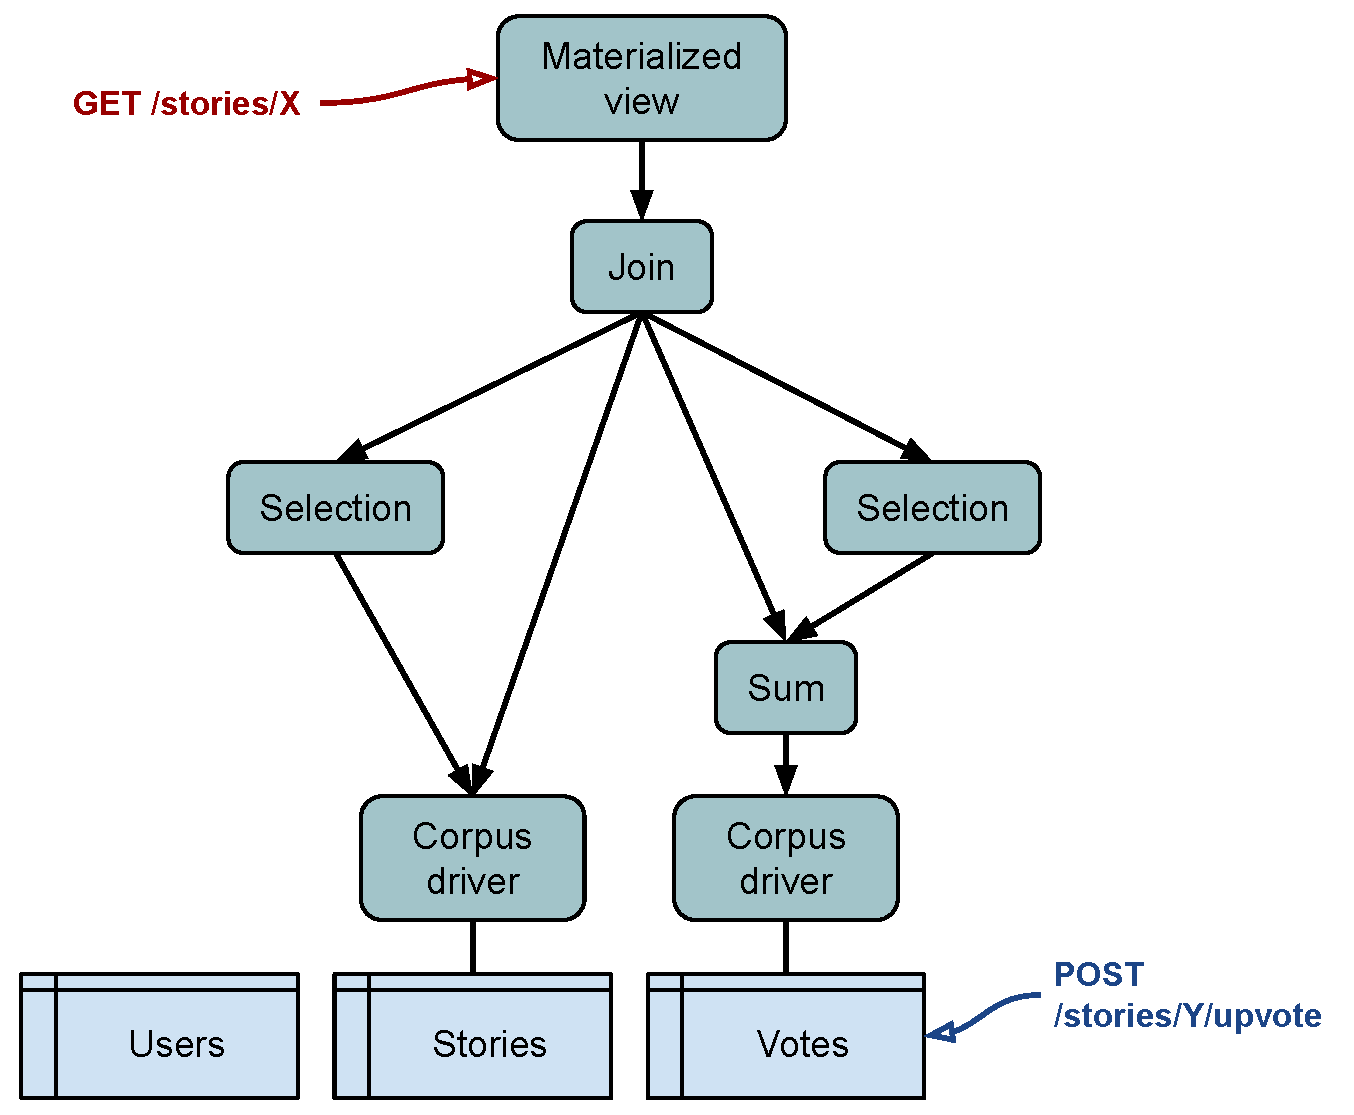
\includegraphics[scale=0.5]{./figures/case_studies/lobsters_architecture_basic.pdf}
  \caption{QPU architecture for the materialized view that integrates vote counts to stories.}
  \label{fig:lobsters_architecture_basic}
\end{figure}

\noindent
The Join QPU in turn generates two downstream queries:

\begin{lstlisting}[
  caption={Quey sent by the Join QPU to the $stories$ Corpus Driver QPU in Figure~\ref{fig:lobsters_architecture_basic}
  during initialization.}
]
Q1 = SELECT id, author_id, title, url
     FROM stories
     INTERVAL FROM LATEST
\end{lstlisting}

\begin{lstlisting}[
  caption={Quey sent by the Join QPU to the Sum QPU in Figure~\ref{fig:lobsters_architecture_basic}
  during initialization.}
]
Q2 = SELECT story_id, SUM(vote)
     FROM votes
     GROUP BY story_id
     INTERVAL FROM LATEST
\end{lstlisting}

\noindent
It sends $Q1$ to the stories Corpus Driver QPU and $Q2$ to the Sum QPU.
We note that it may send the two downstream queries to the corresponding Selection QPUs;
The two query plans are equivalent.

When Join receives $Q1$, it initiates an output stream,
first sending a snapshot of all stories in the stories table,
and then sending an update for each write to the table.

When Sum receives $Q2$, its query processing method sends a downstream query to the votes Corpus Driver QPU
in order to receive the most recent snapshot of the votes table and subscribe to subsequent writes to the table.
As a result, tt receives an input stream consisting of each record in the votes table snapshot,
and incrementally calculates the sum of the $vote$ attribute ($vote\_count$) for each distinct $story\_id$.
Its state is composed of $(story\_id$, $vote\_count)$ tuples.
When the Sum QPU completes processing the snapshot, it emits every computed $(story\_id$, $vote\_count)$ tuple
at its output stream.
In addition, the Sum QPU also receives an input record for each insert to the votes table.
Any update record received while still processing the snapshot, is treaded as a snapshot record;
It updates corresponding $vote\_count$, but does not result to an output record.
For each update received after the votes table snapshot has been processed,
the Sum QPU updates the $vote\_count$ for the corresponding $story\_id$,
and emits the updated $(story\_id$, $vote\_count)$ at its output stream.

Join stores intermediate state for each of input stream.
When it receives an input record from one of the streams,
it matches it with the corresponding stored record for the other stream,
based on the $story\_id$ attribute.

In our implementation of this use case,
the Join QPU is merged with the Materialized View QPU so that the system does not need to maintain state
in order to perform the join operation, in addition to the materialized view state (Section~\ref{sec:eval_scenario}).

In summary,
this QPU architecture provides the functionality of pre-computing story votes counts in order to avoid re-computation
when serving user read requests.
This is equivalent to the functionality already implemented in the Lobsters application.
However, using the QPU-based materialized view shifts the responsibility of updating the vote counts from the application logic,
to the query processing architecture, thus simplifying the application code.


\subsection{Partial materialization}

We expand the Lobsters case study by examining the operation of loading the application's frontpage.
The frontpage consists of the $K$ stories with the highest vote count ($K$ being a parameter).

The Lobsters implementation uses the following query to retrieve the information required for loading the front page:

\begin{lstlisting}[
  basicstyle=\normalfont\ttfamily,
  caption={Query that retrieves the stories in the Lobsters front page.}
  ]
SELECT id, author, title, url, vote_count
FROM stories
JOIN (
  SELECT story_id, SUM(v.vote) as vote_count
	FROM votes
	GROUP BY story_id
) view
ON stories.id = view.story_id
ORDER BY vote_count DESC
LIMIT K
\end{lstlisting}

\begin{figure}[t]
  \centering
    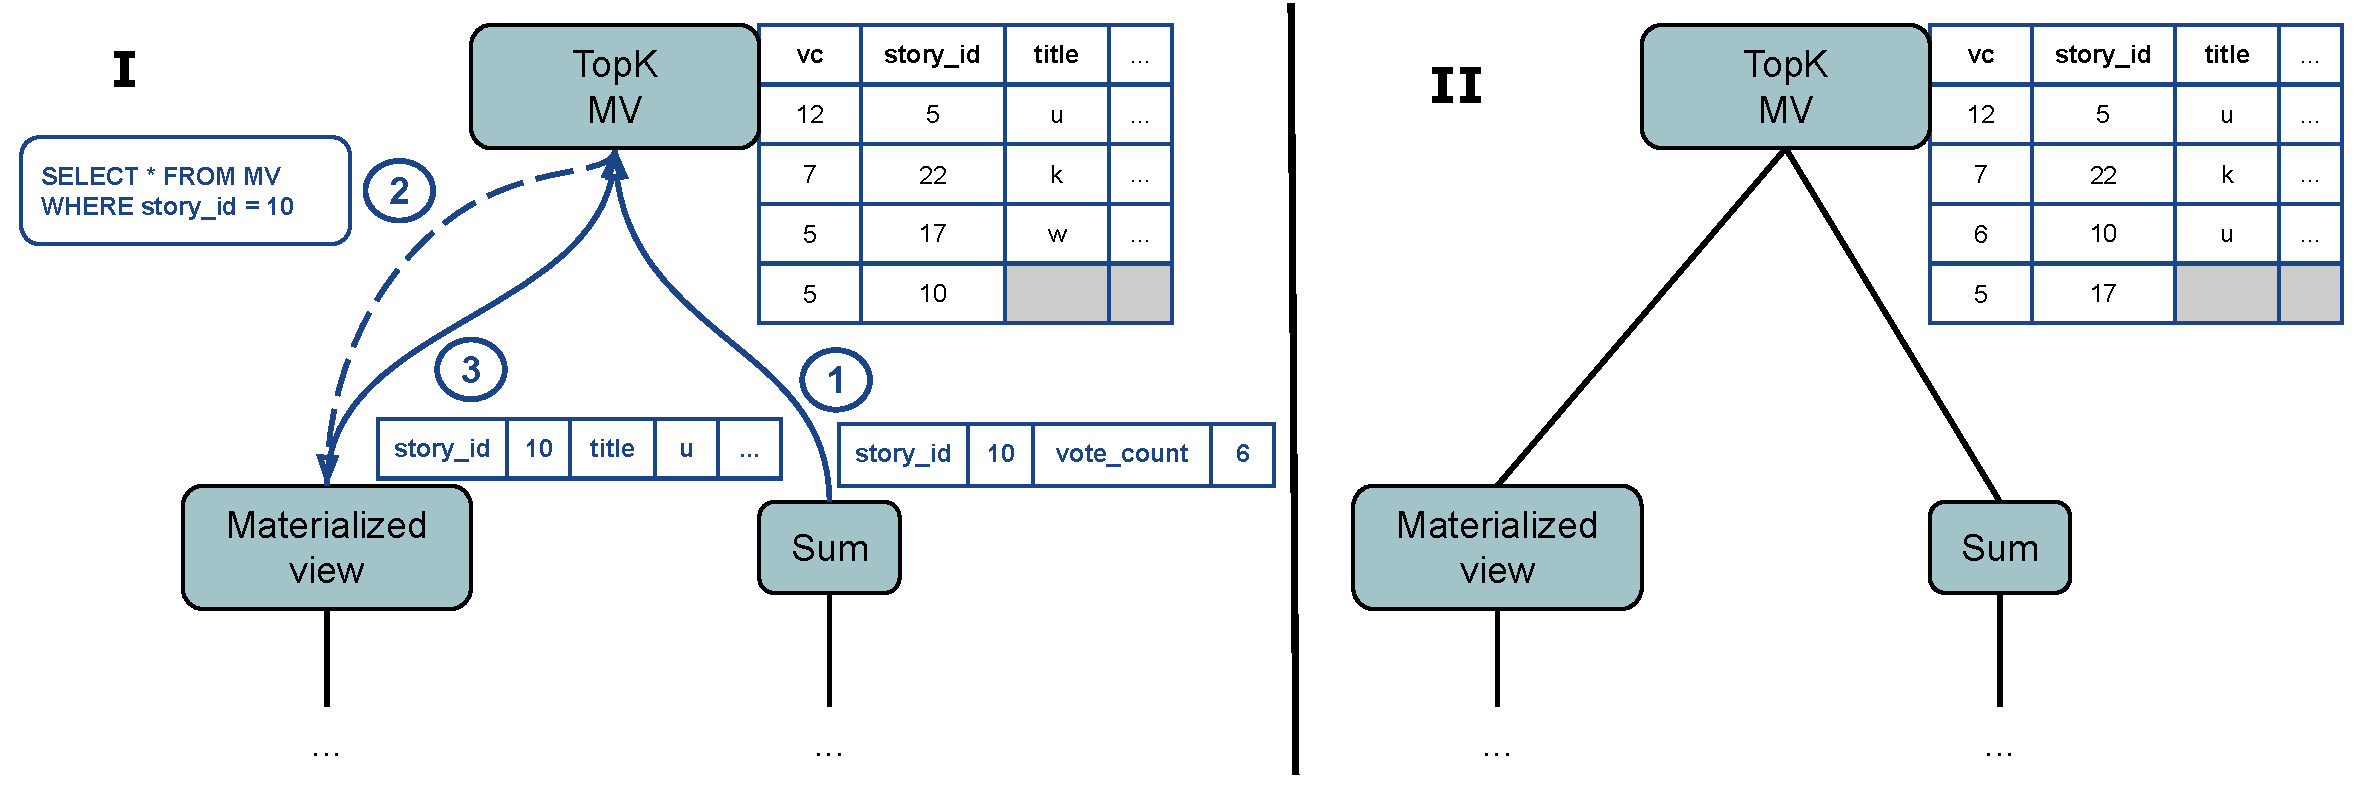
\includegraphics[scale=0.4]{./figures/case_studies/lobsters_architecture_materialization.pdf}
  \caption{A vote triggers the materialization of an entry of the TopK materialized view.}
  \label{fig:lobsters_architecture_materialization}
\end{figure}

In this section, we show how the QPU architecture defined in the previous section can be extended to provide this
functionality.

To achieve that, we introduce an additional query processing unit class: the TopK Materialized View (TopK-MV) QPU.
The TopK-MV represents a materialized view which orders its entries based on a specified attribute.
In addition, it only materializes the $K$ entries with the highest (or lowest) values for that attribute.

We deploy a TopK-MV QPU in the Lobster application QPU architecture (Figure~\ref{fig:lobsters_architecture_materialization}),
and configure it as a materialized view with the same definition as the existing materialized view,
storying entries of the form $(story\_id$, $author\_id$, $title$, $url$, $vote\_count)$.
In addition, we configure TopK-MV QPU to order entries by $vote\_count$, and materialize the $K$ entries with the highest $vote\_count$.

The TopK-MV is connected to the Materialized view QPU and the Sum QPU.
Its initialization method sends a persistent query to the Sum QPU.
As a result, it first receives a snapshot containing the $vote\_count$ of every existing story in snapshot of the votes table;
It subsequently receives an update for each change to the $vote\_count$ of a story.
It stores the received snapshot as a list of $(vote\_count$, $story\_id)$ entries, ordered by $vote\_count$.
Then, for each of the $K$ entries with the highest $vote\_count$,
it sends a downstream query to the Materialized View QPU in order to retrieve the remaining attributes of the corresponding story.
Therefore, the TopK-MV \textit{materializes} a bounded number of entries, based on a given criterion.

Furthermore, the TopK-MV QPU continues receiving updates from the Sum QPU, and updating its
ordered list of $(vote\_count$, $story\_id)$ entries.
When the $vote\_count$ of a non-materialized entry becomes one of the top-K,
the unit's stream processor method discards the materialized entry with the lowest $vote\_count$,
and triggers the materialization of that entry.

The Top-K QPU uses the technique of \textit{partial materialization} in order to bound the size of pre-computed state.
This is a well known concept for materialized views in database systems \cite{zhou:partiallymaterialized, zhou:dynamicmaterialized},
and has been used by Noria \cite{gjengset:noria} in the context of data-flow systems.

\subsection{Placing materialized views at the edge}

% The ad-serving application's users are distributed worldwide, and therefore, the communication latency between user devices and the data center may be significant.
% Placing data geographically closer to end users is a common technique for reducing the large access latencies resulting from geo-distribution 

Query response time is crucial for user-facing read-heavy application, such as Lobsters.
As discussed in chapter~\ref{ch:background}, even small increases in user-perceived latency can result in significant drops in both web traffic and sales.
So far in this case study, we have examined how query response time can be decreased using pre-computed query results.
Another factor contributing to query response time is the communication latency between the application and the clients.
A client located in a different geographic region than the Lobsters application deployment might experience communication
latency in the order of hundreds of milliseconds.

A common solution to this latency problem is to place on servers geographically closer to clients using caches,
in order to avoid costly remote round-trips to data centers.
These servers, called edge nodes, are a crucial component in industry architectures.
For example, Google operates comparatively few data centers relative to edge nodes \cite{google:infra}.
In existing applications,
edge nodes are largely used for caching static data, such as images and video content, for example in content delivery network architectures.

\begin{figure}[t]
  \centering
    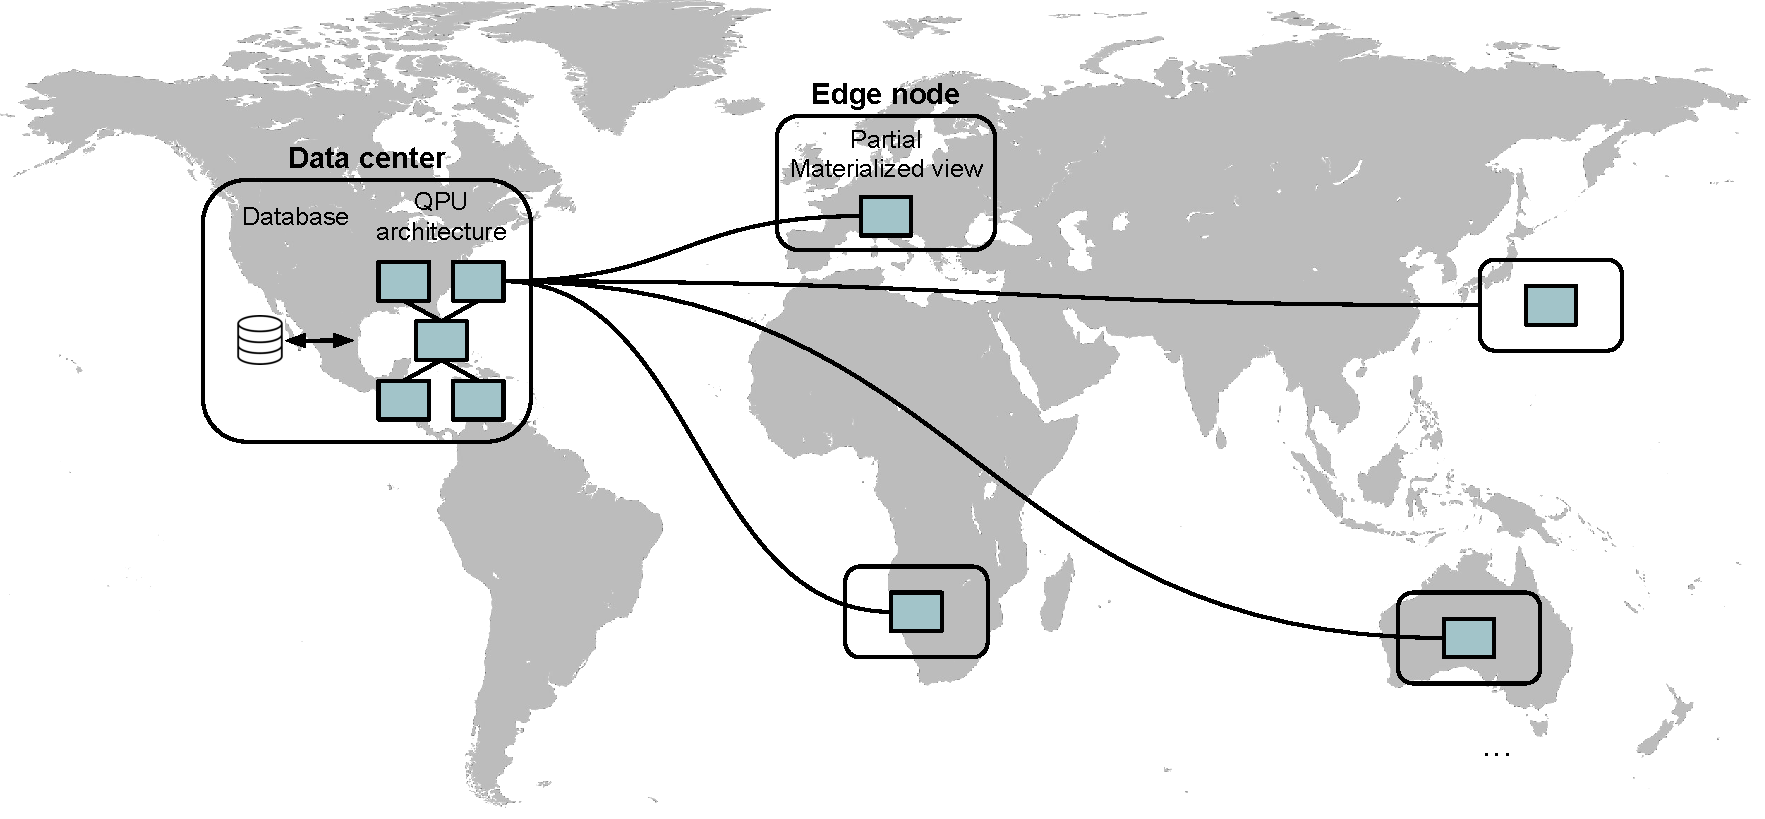
\includegraphics[scale=0.4]{./figures/case_studies/lobsters_architecture_edge.pdf}
  \caption{Distributing a QPU architecture between the data center and edge nodes.}
  \label{fig:lobsters_architecture_edge}
\end{figure}

Because of its modularity, the proposed query processing architecture can be used to place derived state, such as materialized views,
closer to client.
More specifically,
the query architecture designed for the Lobsters application (Figure~\ref{fig:lobsters_architecture_materialization}) can be
distributed among the data centers and edge nodes.
Considering a system architecture composed of a data center and multiple edge nodes,
we can place a TopK Materialized View QPU on each edge node, as shown in Figure~\ref{fig:lobsters_architecture_edge}.
Each TopK-MV QPU stored pre-computed state for the $K$ stories with the most votes.
It thus provides low latency access to the data required for loading the application's frontpage,
while maintaining a bounded memory footprint.
We connect each TopK-MV QPU to the complete Materialized View QPU and the SUM QPU placed in the data center,
In that way, TopK-MV QPUs can receive updates for updated vote counts,
and also request the materialize new stories as the reach the application frontpage.

We configure the connections between each TopK-MV QPU and the QPU architecture placed on the data center to be asynchronous,
as propagating each vote to the edge nodes synchronously adds a significant overhead to vote operations.
This choice makes a trade-off between write latency and the freshness of materialized views.
Propagating updates to materialized views asynchronously means that views are eventually consistent,
and might therefore return stale results.

In chapter~\ref{ch:evaluation}, we evaluate the effect of placing materialized view closer to clients on query response time and
and query result freshness.